\documentclass[border=3pt]{standalone}
\usepackage{fontspec}
\setmainfont{Times New Roman}
\usepackage{pgfplots}
\pgfplotsset{compat=1.18}
\usetikzlibrary{arrows.meta,calc,positioning,shapes.geometric}
\definecolor{forest}{HTML}{346E57}
\definecolor{sage}{HTML}{E8EFEA}
\definecolor{clay}{HTML}{B77E60}
\definecolor{gray}{HTML}{718078}
\definecolor{rule}{HTML}{B7C3BA}
\definecolor{ink}{HTML}{000000}
\begin{document}
\hyphenpenalty=10000\exhyphenpenalty=10000
\fontsize{10}{12}\selectfont
\renewcommand{\small}{\fontsize{9}{11}\selectfont}
\renewcommand{\scriptsize}{\fontsize{8}{10}\selectfont}
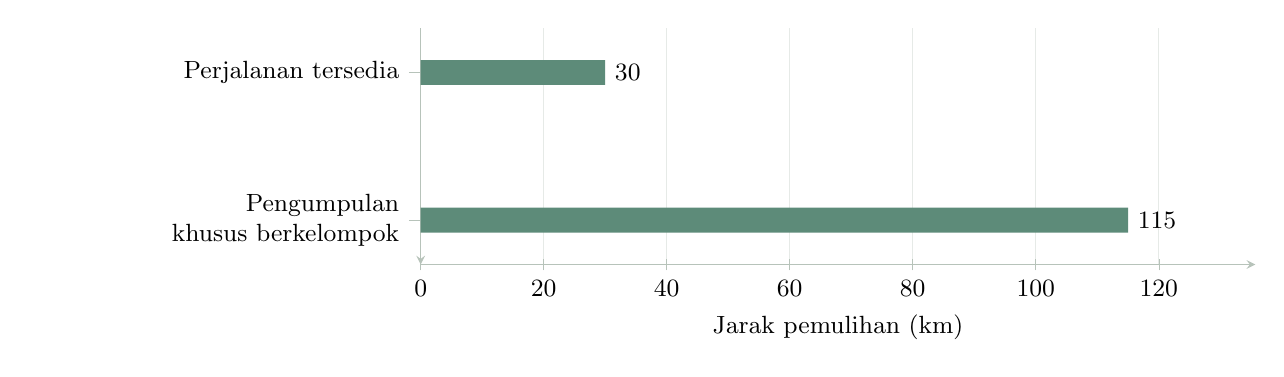
\begin{tikzpicture}\begin{axis}[width=10.6cm,height=3cm,scale only axis=true,
axis lines=left,axis line style={draw=rule},tick style={draw=rule},
tick label style={font=\small},label style={font=\small},
grid=major,grid style={draw=rule!35,line width=.3pt},
legend style={draw=none,fill=none,font=\small,at={(.5,-.26)},anchor=north},legend columns=-1,
xbar,bar width=9pt,xmin=0,xmax=135.7,enlarge y limits=.3,y dir=reverse,ytick={0,1},yticklabels={{Perjalanan tersedia},{Pengumpulan khusus berkelompok}},yticklabel style={text width=4.6cm,align=right},xlabel={Jarak pemulihan (km)},ymajorgrids=false,nodes near coords,point meta=x,nodes near coords align={horizontal},every node near coord/.append style={font=\small,text=ink},]
\addplot[draw=none,fill=forest!80] coordinates {(30,0) (115,1)};
\end{axis}\end{tikzpicture}
\end{document}
